\documentclass{article}
\usepackage{amsmath, amssymb, graphicx, subfigure, algorithmic, color}

\author{Mitchell Koch, Justin Huang}
\title{Learning Relation Entailment Graphs\\CSE 515 Final Report}
\date{Friday, June 14, 2013}

\begin{document}
\maketitle

\begin{abstract}
Can learning relation entailment graphs based on WordNet or Bayes net
structure learning improve relation query performance?
\end{abstract}

\section{Introduction and Motivation}

Open IE~\cite{Etzioni:2008:OIE:1409360.1409378}

previous relation entailment
work~\cite{Berant:2012:LER:2122944.2122947, berant2011global}, on work in relation
extraction using matrix factorization~\cite{riedel13relation}, 

as well as on related work in probabilistic modeling of relations
between entities~\cite{TaskarWAK03, Taskar:2002:DPM:2073876.2073934}.

Freebase using distant supervision as in~\cite{HoffmannZLZW11}

\subsection{Database Query Task}
We define the following database query task to evaluate a relation entailment graph. Let $R$ be a set of relation strings, and $A$ be a set of argument strings. We are given a database $D$ of facts, where each fact is of the form $r(x, y)$ for some $r\in R$ and $x, y\in A$.

Given a query for a relation $r$ with arguments $x$ and $y$, we can expand the query to additionally search for all $r^\prime(x, y)$ such that there exists an edge from $r^\prime$ to $r$ in the entailment graph. An example of this process is shown in Figure~\ref{query-expansion}. We can then evaluate the correctness of the returned results.

\begin{figure}[h]
\begin{center}
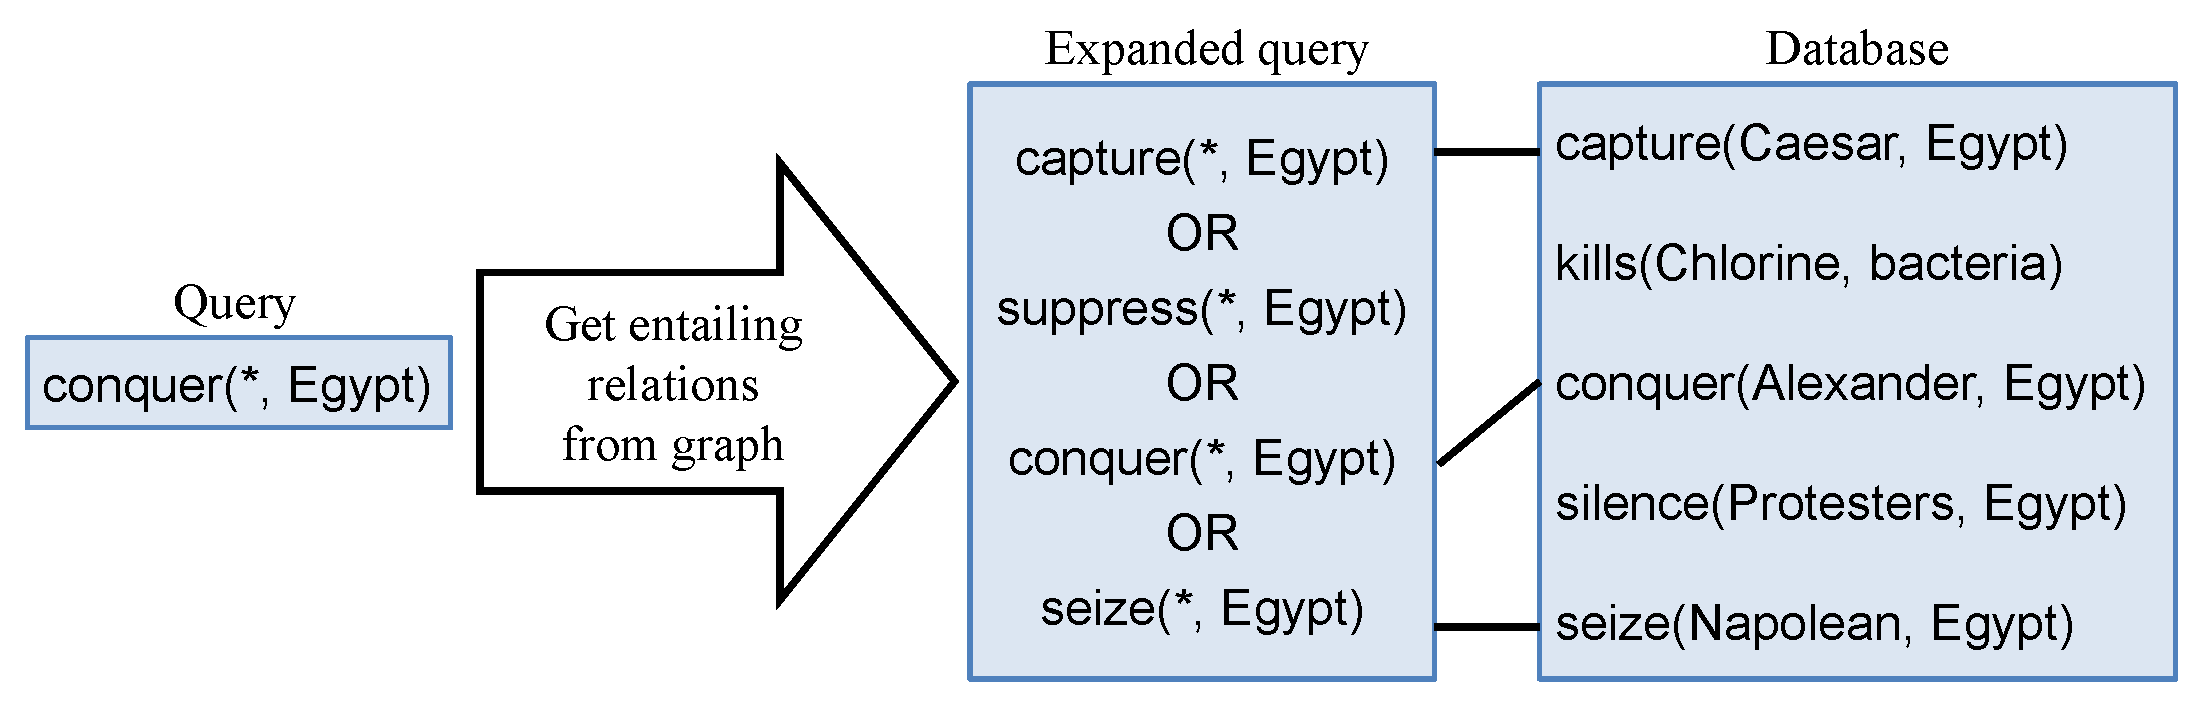
\includegraphics[width=1.0\textwidth]{figures/query-expansion.pdf}
\end{center}
\caption{An example of a query being expanded.}\label{query-expansion}
\end{figure}

\section{Methods and Algorithms}

\subsection{Constraints on WordNet}

WordNet~\cite{fellbaum98wordnet} is a hand-crafted resource that distinguishes between different word senses, and provides synonyms and entailments between them. We denote a WordNet sense with a number where \textit{\#1} is the most common. For example \textit{note\#4} is the fourth most common sense of ``note,'' which means ``to write down''. Each WordNet sense has its sense number, a count indicating how often that sense is used, and a probability, which is the count divided by the sum of counts for all senses of the same word.

\subsubsection{WordNet entailment graph}
A troponym is a specialization of a word, e.g., ``to fly'' is a troponym of ``to travel.'' We say that WordNet sense $w_1$ entails $w_2$ if $w_1$ is a synonym of $w_2$, if $w_1$ is a troponym of $w_2$ in WordNet, or if there exists some $w_3$ such that $w_1$ entails $w_3$ and $w_3$ entails $w_2$. A path in the entailment graph is defined as the sequence of troponyms between $w_1$ and $w_2$. The entailment graph is disconnected. Figure ~\ref{wordnet-graph} shows one component of the graph, and Figure ~\ref{example-path} shows an example of a path in the graph, from \textit{note\#4} to \textit{write\#2}.

Although WordNet already defines an entailment graph between verb senses, one hurdle to using it is determining what sense to use. For example, given the verb ``take,'' is it \textit{take\#21} (take by force) or \textit{take\#2} (take time)? Each sense will lead to very different entailments. The first part of our approach is to assume a string can take on any of its WordNet senses, which may lead to noisier entailments. The second part is to train a logistic regression classifier to help filter out noisy entailments.

\subsubsection{Logistic regression classifier}
For a certain training set of queries, we use all possible entailments from WordNet on the database query task, and label each fact as relevant to the query or not relevant to the query. We use these results as training data. For each result, we record the path that was taken in the entailment graph and produce the following features:
\begin{enumerate}
  \item Path length
  \item Average sense number
  \item Average WordNet probability
  \item Maximum sense number
  \item Minimum WordNet probability
\end{enumerate}

The length of the path is how many nodes there were in the path. For example, in figure ~\ref{example-path}, the length is 3. Because WordNet senses are ranked in order frequency, we use the average and maximum sense numbers as features, the idea being that an uncommon WordNet sense (e.g., \textit{take\#42}) could be a weak link in the entailment path. A similar intuition holds for the probabilities of the WordNet senses.

The output of logistic regression is a set of weights $w$ for each feature. Let $x$ be the vector of features described above. Then the probability of the label we would like to predict is given by:
\begin{align*}
  p(x) = \frac{e^{w\cdot x}}{1 + e^{w\cdot x}}
\end{align*}

Finally, we run the database query task on the test set of queries, using the learned model to filter out unlikely entailments.

\begin{figure}[h]
\begin{center}
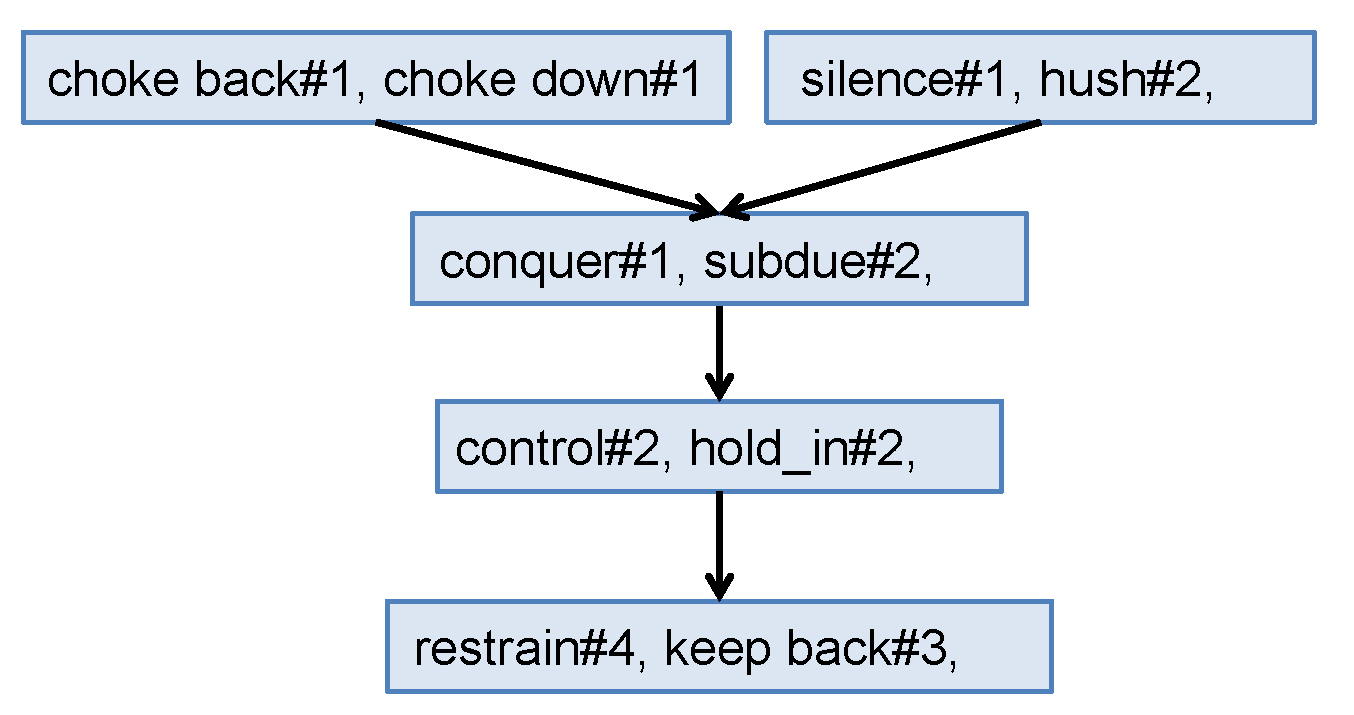
\includegraphics[width=0.6\textwidth]{figures/wordnet-graph.pdf}
\end{center}
\caption{Component of the WordNet entailment graph with the first sense of conquer, \textit{conquer\#1}. Boxes represent synonym sets, arrows represent entailments.}\label{wordnet-graph}
\end{figure}

\begin{figure}[h]
\begin{center}
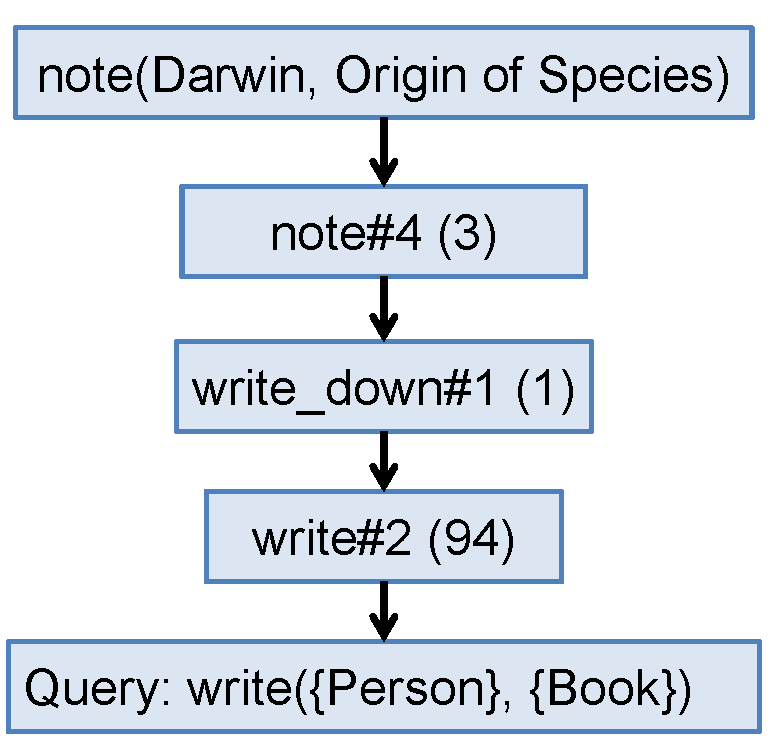
\includegraphics[width=0.4\textwidth]{figures/example-path.pdf}
\end{center}
\caption{Example path in entailment graph}\label{example-path}
\end{figure}


\subsection{Bayesian Network Structure Learning}

\begin{figure}[h]
\begin{center}
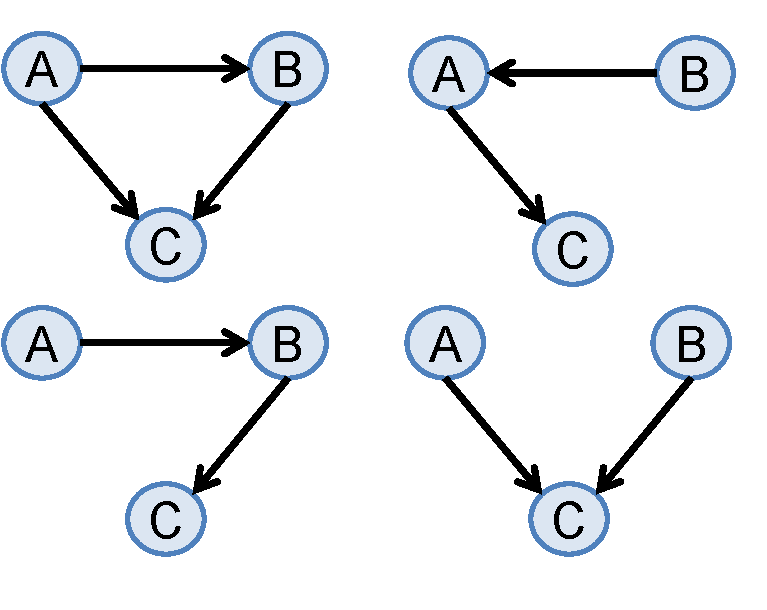
\includegraphics[width=0.4\textwidth]{figures/example-net-structures.pdf}
\end{center}
\caption{Examples of possible network structures}\label{example-net-structures}
\end{figure}


\section{Experiments and Results}

\section{Discussion and Conclusion}


\bibliographystyle{abbrv}
\bibliography{bib}

\end{document}
